%%***********************************************
%% Plantilla para TFG.
%% Escuela Técnica Superior de Ingenieros Informáticos. UPM.
%%***********************************************
\documentclass[a4paper,11pt]{book}

%%-----------------------------------------------
%% Importar Preámbulo:
% -*-coding: utf-8 -*-
%%***********************************************
%% Plantilla para TFG.
%% Escuela Técnica Superior de Ingenieros Informáticos. UPM.
%%***********************************************
%% Preámbulo del documento.
%%***********************************************
\usepackage[T1]{fontenc}
\usepackage[utf8]{inputenc}
\usepackage[english,spanish,es-lcroman]{babel}
\usepackage{bookman}
\decimalpoint
\usepackage{graphicx}

\usepackage{amsfonts,amsgen,amsmath,amssymb}
\usepackage[top=3.5cm, bottom=3.5cm, right=3cm, left=3cm]
{geometry}
\usepackage{afterpage}
\usepackage{colortbl,longtable}
\usepackage[pdfborder={0 0 0},pdfusetitle]{hyperref}
\usepackage{pdfpages}
\usepackage{url}
\usepackage[stable]{footmisc}
\usepackage{parskip} % para separar párrafos con espacio.
%%-----------------------------------------------
\usepackage{fancyhdr}
\pagestyle{fancy}
\fancyhf{}
\fancyhead[LO]{\leftmark}
\fancyhead[RE]{\rightmark}
\setlength{\headheight}{1.5\headheight}
\cfoot{\thepage}

\addto\captionsspanish{ \renewcommand{\contentsname}
  {Tabla de contenidos} }
\setcounter{tocdepth}{4}
\setcounter{secnumdepth}{4}

\renewcommand{\chaptermark}[1]{\markboth{\textbf{#1}}{}}
\renewcommand{\sectionmark}[1]{\markright{\textbf{\thesection. #1}}}
\newcommand{\HRule}{\rule{\linewidth}{0.5mm}}
\newcommand{\bigrule}{\titlerule[0.5mm]}

\usepackage{appendix}
\renewcommand{\appendixname}{Anexos}
\renewcommand{\appendixtocname}{Anexos}
%\renewcommand{\appendixpagename}{Anexos}
%%-----------------------------------------------
%% Páginas en blanco sin cabecera:
%%-----------------------------------------------
\usepackage{dcolumn}
\newcolumntype{.}{D{.}{\esperiod}{-1}}
\makeatletter
\addto\shorthandsspanish{\let\esperiod\es@period@code}

\def\clearpage{
  \ifvmode
    \ifnum \@dbltopnum =\m@ne
      \ifdim \pagetotal <\topskip
        \hbox{}
      \fi
    \fi
  \fi
  \newpage
  \thispagestyle{empty}
  \write\m@ne{}
  \vbox{}
  \penalty -\@Mi
}
\makeatother

%%-----------------------------------------------
%% Configuración relacionada con la accesibilidad del documento PDF
%% (tagged PDF).
%%-----------------------------------------------
% Comentado porque tiene algunos issues relacionados con lineno y texto formateado en headers
% \usepackage{accessibility}

\graphicspath{{imagenes/}}

%% -----------------------------------------------
%% Cargar datos relativos al TFG:
%% (actualizar estos datos en ./datos_tfg.tex)
%%***********************************************
%% Plantilla para TFG.
%% Escuela Técnica Superior de Ingenieros Informáticos. UPM.
%%***********************************************
%% Información requerida para completar la portada.
%%***********************************************

%% Escribe Nombre y Apellidos del autor del trabajo:
\newcommand{\NombreAutor}{Jan Cerezo Pomykol}

%% Escribe el Grado:
\newcommand{\Grado}{Ingeniería Informática}

%% Escribe el Título del Trabajo:
\newcommand{\TituloTFG}{Cuadro de Mandos para Visualizar Algoritmos Distribuidos}

%% Escribe Nombre y Apellidos del Tutor del trabajo:
\newcommand{\NombreTutor}{Fernando Pérez Costoya}

% Escribe el Departamento al que pertenece el Tutor:
\newcommand{\Departamento}{Departamanto de Arquitectura y Sistemas Informáticos}

% Escribe la fecha de lectura, en formato: Mes - Año
\newcommand{\Fecha}{Abril - 2022}

% Establecer los datos con los comandos estándares de LaTeX
\title{\TituloTFG}
\author{\NombreAutor}
\date{\Fecha}
%%***********************************************


%% -----------------------------------------------
%% Importación de otros paquetes de LaTeX a usar en el desarrollo del TFG:
%% (veanse algunos ejemplos como listings (para incluir código), todonotes (para poner anotaciones al margen con cosas por hacer), etc.
%%-----------------------------------------------
\usepackage{color}

\definecolor{gray97}{gray}{.97}
\definecolor{gray75}{gray}{.75}
\definecolor{gray45}{gray}{.45}

\usepackage{listings}
\lstset{ frame=Ltb,
     framerule=0pt,
     aboveskip=0.5cm,
     framextopmargin=3pt,
     framexbottommargin=3pt,
     framexleftmargin=0.4cm,
     framesep=0pt,
     rulesep=.4pt,
     backgroundcolor=\color{gray97},
     rulesepcolor=\color{black},
     %
     stringstyle=\ttfamily,
     showstringspaces = false,
     basicstyle=\scriptsize\ttfamily,
     commentstyle=\color{gray45},
     keywordstyle=\bfseries,
     %
     numbers=left,
     numbersep=6pt,
     numberstyle=\tiny,
     numberfirstline = false,
     breaklines=true,
   }
\lstnewenvironment{listing}[1][]
   {\lstset{#1}\pagebreak[0]}{\pagebreak[0]}

\lstdefinestyle{consola}
   {basicstyle=\scriptsize\bf\ttfamily,
    backgroundcolor=\color{gray75},
    }

\lstdefinestyle{CodigoC}
   {basicstyle=\scriptsize,
	frame=single,
	language=C,
	numbers=left
   }

\lstdefinestyle{CodigoC++}
   {basicstyle=\small,
	frame=single,
	backgroundcolor=\color{gray75},
	language=C++,
	numbers=left
   }

\lstdefinestyle{Python}
   {language=Python,
   }


\usepackage[textwidth=2.5cm, textsize=smaller]{todonotes}
\setlength{\marginparwidth}{2.5cm}
\setlength{\parindent}{2em}

\usepackage{lipsum}

\usepackage{relsize}

\usepackage{svg}
\usepackage{amsmath}
\usepackage{calc}
\usepackage{float}


%%-----------------------------------------------
%% Documento:
\begin{document}
%%***********************************************
%% Plantilla para TFG.
%% Escuela Técnica Superior de Ingenieros Informáticos. UPM.
%%***********************************************
%% Portada.
%%***********************************************
\begin{titlepage}

\begin{minipage}{0.15\linewidth}
\hspace*{-2.5cm}
\noindent

\includegraphics[scale=0.5]{include/escudo_upm.png} \qquad\qquad
\end{minipage}
\begin{minipage}{0.7\linewidth}
\begin{center}
\huge{ Universidad Politécnica\\de Madrid }\\
\vspace*{0.5cm}
\Large{\textbf{Escuela Técnica Superior de \\
Ingenieros Informáticos}}
\end{center}
\end{minipage}
\begin{minipage}{0.2\linewidth}

\includegraphics[scale=0.5]{include/escudo_etsiinf.png}
\end{minipage}

\vspace*{1cm}
\begin{center}
\Large{Grado en  \Grado{} }
\end{center}

\vspace*{1cm}
\begin{center}
\huge{ Trabajo Fin de Grado }
\end{center}

\vspace*{0.5cm}
\begin{center}
\huge\bfseries {  \TituloTFG{} }
\end{center}

\vspace*{5cm}

\noindent
\large{Autor: \NombreAutor{} }\\
\large{Tutor: \NombreTutor{} }


\vspace*{3cm}
\begin{center}
Madrid, \Fecha
\end{center}

%%--------------------------------
\newpage
\thispagestyle{empty}
%%--------------------------------
\noindent
Este Trabajo Fin de Grado se ha depositado en la ETSI Informáticos de la Universidad Politécnica de Madrid para su defensa.

\vspace*{4cm}
\noindent
\textit{Trabajo Fin de Grado}\\
\textit{Grado en} \Grado{}

\begin{enumerate}
\item[\textit{Título:}] \TituloTFG{}
\end{enumerate}
\Fecha


\vspace*{3cm}

\noindent
\begin{tabular}{ll}
\textit{Autor:} & \NombreAutor{}  \\
\textit{Tutor:} & \NombreTutor{}  \\
                & \Departamento{} \\
                & ETSI Informáticos\\
                & Universidad Politécnica de Madrid
\end{tabular}

\end{titlepage}


%%-----------------------------------------------
%% Numeración romana:
\frontmatter
%%-----------------------------------------------
\chapter*{Resumen}

Cuando se habla de sistemas distribuidos, una de las propiedades fundamentales de los algoritmos de esta disciplina es que se ejecutan en múltiples máquinas (nodos) concurrentemente. Estos nodos interactúan de alguna manera entre ellos para lograr un objetivo determianado. Por lo general, la simultaneidad de los eventos causa dificultades a los estudiantes de la materia a la hora de entender el funcionamiento de estos algoritmos puesto que es complicado mantener una visión global del estado del sistema.

Este proyecto tiene como objetivo principal proporcionar una herramienta que facilite la comprensión del funcionamiento de los algoritmos de la asignatura de Sistemas Distribuidos. A diferencia de otras implementaciones que simplemente visualizan una simulación el algoritmo, en esta se pretende visualizar una ejecución real. De esta forma se podrá también ofrecer la posibilidad de interactuar con los nodos en tiempo de ejecución, pudiendo observar cómo el algoritmo reacciona ante distintas situaciones. Además de ofrecer una solución que facilita el aprendizaje en la asignatura de Sistemas Distribuidos, también se podría emplear como una herramienta de depuración de estos algoritmos.

\newpage

\chapter*{Abstract}

When it comes to distributed systems, one of the most important aspects of the algorithms is that they are executed simultaneously in various independent machines, commonly referred as nodes. These nodes interact with each other to achieve some objective. The simultaneousness of the events usually causes difficulties to the students when they try to understand the behavior of the algorithm. This is due to the fact that it is hard to maintain a global vision of the state of the distributed system.

The main goal of this project is to provide a tool that facilitates the understanding of the algorithms of the distributed system discipline. Contrary to other existing implementations that only simulate a visualization of the algorithm, this one will visualize a real execution, permitting real-time interaction with the nodes. This allows to visualize how the algorithm reacts in different situations. Additionally, this tool provides a debugging environment for this type of algorithms.


%%%%%%%%%%%%%%%%%%%%%%%%%%%%%%%%%%%%%%%%%%%%%%%%%%%%%%%%%%%
%% Final del resumen. 
%%%%%%%%%%%%%%%%%%%%%%%%%%%%%%%%%%%%%%%%%%%%%%%%%%%%%%%%%%%
\tableofcontents

%%-----------------------------------------------
%% Contenido del TFG
\chapter{Resumen del trabajo realizado}
\label{ch:trabajo_realizado}

Inicialmente el plan de trabajo tenía como objetivo resolver las tareas de la tabla~\ref{lista_tareas}, dedicando las horas indicadas.

\begin{table}[h]
\centering
\begin{tabular}{|p{1cm}|p{11cm}|p{1.1cm}|}
\hline
\textbf{Num} & \textbf{Tarea} & \textbf{Horas}\\
\hline\hline
1 & Formación en tecnologías de visualización y lenguajes de programación necesarios. & 90\\
\hline
2 & Selección e implementación del algoritmo a visualizar. & 30\\
\hline
3 & Diseño de la interacción del cuadro de mandos con el algoritmo a visualizar. & 10\\
\hline
4 & Implementación y pruebas del cuadro de mandos. & 120\\
\hline
5 & Elaboración de la memoria. & 45\\
\hline
6 & Elaboración de la presentación. & 10\\
\hline
7 & Preparación de la defensa del trabajo. & 19\\
\hline\hline
\textbf{} & \textbf{Total} & \textbf{324}\\
\hline
\end{tabular}
\caption{Lista de tareas}
\label{lista_tareas}
\end{table}

La planificación inicial contaba con la distribución de tareas por semanas que se muestra en el diagrama de Gantt de la Figura~\ref{plan_trabajo}. Cabe resaltar que la dedicación por semanas de cada tarea no es representativa de las horas semanales dedicadas a dicha tarea. El diagrama es una imagen con formato \texttt{svg}, por tanto se puede aumentar para leer con claridad el contenido.

\begin{figure}[h]
	{\fontsize{3}{4}\selectfont
		\centering
    	\def\svgscale{0.185}
    	\input{imagenes/plan_trabajo.pdf_tex}
    	\caption{Diagrama de Gantt planificado}
    	\label{plan_trabajo}
	}
\end{figure}

\newpage

A fecha de escritura (semana del 18 de abril) el diagrama de Gantt correspondiente a las tareas realizadas hasta la fecha es el de la Figura~\ref{trabajo_realizado}.

\begin{figure}[H]
	{\fontsize{3}{4}\selectfont
		\centering
    	\def\svgscale{0.185}
    	\chapter{Resumen del trabajo realizado}
\label{ch:trabajo_realizado}

Inicialmente el plan de trabajo tenía como objetivo resolver las tareas de la tabla~\ref{lista_tareas}, dedicando las horas indicadas.

\begin{table}[h]
\centering
\begin{tabular}{|p{1cm}|p{11cm}|p{1.1cm}|}
\hline
\textbf{Num} & \textbf{Tarea} & \textbf{Horas}\\
\hline\hline
1 & Formación en tecnologías de visualización y lenguajes de programación necesarios. & 90\\
\hline
2 & Selección e implementación del algoritmo a visualizar. & 30\\
\hline
3 & Diseño de la interacción del cuadro de mandos con el algoritmo a visualizar. & 10\\
\hline
4 & Implementación y pruebas del cuadro de mandos. & 120\\
\hline
5 & Elaboración de la memoria. & 45\\
\hline
6 & Elaboración de la presentación. & 10\\
\hline
7 & Preparación de la defensa del trabajo. & 19\\
\hline\hline
\textbf{} & \textbf{Total} & \textbf{324}\\
\hline
\end{tabular}
\caption{Lista de tareas}
\label{lista_tareas}
\end{table}

La planificación inicial contaba con la distribución de tareas por semanas que se muestra en el diagrama de Gantt de la Figura~\ref{plan_trabajo}. Cabe resaltar que la dedicación por semanas de cada tarea no es representativa de las horas semanales dedicadas a dicha tarea. El diagrama es una imagen con formato \texttt{svg}, por tanto se puede aumentar para leer con claridad el contenido.

\begin{figure}[h]
	{\fontsize{3}{4}\selectfont
		\centering
    	\def\svgscale{0.185}
    	\input{imagenes/plan_trabajo.pdf_tex}
    	\caption{Diagrama de Gantt planificado}
    	\label{plan_trabajo}
	}
\end{figure}

\newpage

A fecha de escritura (semana del 18 de abril) el diagrama de Gantt correspondiente a las tareas realizadas hasta la fecha es el de la Figura~\ref{trabajo_realizado}.

\begin{figure}[H]
	{\fontsize{3}{4}\selectfont
		\centering
    	\def\svgscale{0.185}
    	\chapter{Resumen del trabajo realizado}
\label{ch:trabajo_realizado}

Inicialmente el plan de trabajo tenía como objetivo resolver las tareas de la tabla~\ref{lista_tareas}, dedicando las horas indicadas.

\begin{table}[h]
\centering
\begin{tabular}{|p{1cm}|p{11cm}|p{1.1cm}|}
\hline
\textbf{Num} & \textbf{Tarea} & \textbf{Horas}\\
\hline\hline
1 & Formación en tecnologías de visualización y lenguajes de programación necesarios. & 90\\
\hline
2 & Selección e implementación del algoritmo a visualizar. & 30\\
\hline
3 & Diseño de la interacción del cuadro de mandos con el algoritmo a visualizar. & 10\\
\hline
4 & Implementación y pruebas del cuadro de mandos. & 120\\
\hline
5 & Elaboración de la memoria. & 45\\
\hline
6 & Elaboración de la presentación. & 10\\
\hline
7 & Preparación de la defensa del trabajo. & 19\\
\hline\hline
\textbf{} & \textbf{Total} & \textbf{324}\\
\hline
\end{tabular}
\caption{Lista de tareas}
\label{lista_tareas}
\end{table}

La planificación inicial contaba con la distribución de tareas por semanas que se muestra en el diagrama de Gantt de la Figura~\ref{plan_trabajo}. Cabe resaltar que la dedicación por semanas de cada tarea no es representativa de las horas semanales dedicadas a dicha tarea. El diagrama es una imagen con formato \texttt{svg}, por tanto se puede aumentar para leer con claridad el contenido.

\begin{figure}[h]
	{\fontsize{3}{4}\selectfont
		\centering
    	\def\svgscale{0.185}
    	\input{imagenes/plan_trabajo.pdf_tex}
    	\caption{Diagrama de Gantt planificado}
    	\label{plan_trabajo}
	}
\end{figure}

\newpage

A fecha de escritura (semana del 18 de abril) el diagrama de Gantt correspondiente a las tareas realizadas hasta la fecha es el de la Figura~\ref{trabajo_realizado}.

\begin{figure}[H]
	{\fontsize{3}{4}\selectfont
		\centering
    	\def\svgscale{0.185}
    	\input{imagenes/trabajo_realizado.pdf_tex}
    	\caption{Diagrama de Gantt con tareas completadas}
    	\label{trabajo_realizado}
	}
\end{figure}

En este diagrama se pueden observar las semanas en las que se ha trabajado (color verde) o no (color naranja) en determinadas tareas. Como se puede observar, tanto la primera tarea como la tercera están completadas. En cuanto a la cuarta tarea, no se ha trabajado durante las dos primeras semanas puesto que, entre otros factores, se ha tenido que invertir ese tiempo en formación adicional en contenidos relativos a la misma.

    	\caption{Diagrama de Gantt con tareas completadas}
    	\label{trabajo_realizado}
	}
\end{figure}

En este diagrama se pueden observar las semanas en las que se ha trabajado (color verde) o no (color naranja) en determinadas tareas. Como se puede observar, tanto la primera tarea como la tercera están completadas. En cuanto a la cuarta tarea, no se ha trabajado durante las dos primeras semanas puesto que, entre otros factores, se ha tenido que invertir ese tiempo en formación adicional en contenidos relativos a la misma.

    	\caption{Diagrama de Gantt con tareas completadas}
    	\label{trabajo_realizado}
	}
\end{figure}

En este diagrama se pueden observar las semanas en las que se ha trabajado (color verde) o no (color naranja) en determinadas tareas. Como se puede observar, tanto la primera tarea como la tercera están completadas. En cuanto a la cuarta tarea, no se ha trabajado durante las dos primeras semanas puesto que, entre otros factores, se ha tenido que invertir ese tiempo en formación adicional en contenidos relativos a la misma.


\chapter*{Explicación y justificación de las modificaciones del Plan de Trabajo}

El plan de trabajo se mantiene. Sin embargo, el retraso en la cuarta tarea implica que hasta la fecha prevista de finalización de la misma se tendrá que priorizar el progreso en esta. El retraso se debe, en parte, a la gran cantidad de tiempo que se tiene que dedicar a la formación en las tecnologías necesarias. En la implementación se emplean diversos lenguajes de programación y \textit{frameworks} de los cuales, la mayoría, eran desconocidos. Además de este aspecto, el diseño de la interacción del cuadro de mandos con el algoritmo (la parte más difícil de diseñar) ha sufrido numerosas modificaciones que afectan, con mayor o menor medida, a las demás partes de la aplicación.

\section{Revisión de la lista de objetivos del trabajo}

Los objetivos del trabajo se mantienen. A modo de recordatorio, el objetivo principal es proporcionar una herramienta que facilite la comprensión del funcionamiento de los algoritmos de sistemas distribuidos. Esta herramienta debe permitir al usuario interactuar con el algoritmo en tiempo real para poder observar cuál es la reacción ante distintas situaciones. El proyecto, además de tener un objetivo pedagógico, también puede ser empleado con fines de depuracion por los desarrolladores de estos algoritmos.

\section{Revisión de la lista de tareas}

Tanto la lista de tareas como las horas de dedicación a las mismas se mantiene. Se puede consultar en el cuadro del \hyperref[ch:trabajo_realizado]{capítulo anterior}.

\newpage

\section{Revisión del Diagrama de Gantt}

La distribución de las tareas por semanas se mantiene, puede consultarse en el diagrama de la Figura~\ref{revision_gantt}.

\begin{figure}[H]
	{\fontsize{3}{4}\selectfont
		\centering
    	\def\svgscale{0.26}
    	\input{imagenes/revision_gantt.pdf_tex}
    	\caption{Diagrama de Gantt revisado}
    	\label{revision_gantt}
	}
\end{figure}


%%-----------------------------------------------
%% Numeración arábiga:
\mainmatter

\chapter{Introducción}
\label{ch:intro}

Uno de los aspectos más dificultosos para los estudiantes de la disciplina de sistemas distribuidos es comprender el modo de operación de los algoritmos propuestos en esta materia. La simultaneidad de los eventos en los nodos dificulta mantener una comprensión del estado global del algoritmo. A esto se le suma complejidad que supone la caída de nodos o el comportamiento anómalo de estos. Este proyecto proporciona una herramienta que facilita la comprensión del estado del algoritmo mediante la visualización de los nodos del sistema y los mensajes entre estos. Esta herramienta no sólo puede ser empleada con fines docentes, si no también con fines de depuración de algoritmos distribuidos.

\section{Trabajos previos}

En la actualidad ya existen numerosas implementaciones que logran este tipo de visualizaciones. No obstante, se pueden clasificar en dos conjuntos:

\begin{enumerate}
\item Las que ejecutan una simulación. Los nodos del sistema distribuido no son ``reales``, si no que se simula el comportamiento con fines meramente visuales. Algunos ejemplos de este tipo son \cite{raft1}, \cite{raft2}, \cite{raft3}.
\item Las que visualizan una ejecución real. En estas implementaciones los nodos sí son procesos reales que se ejecutan localmente o en un servidor. El entorno de visualización captura, de alguna manera, los mensajes entre nodos para visualizar el estado de cada uno. Un ejemplo de este tipo es \cite{MOSES200497}.
\end{enumerate}

Sin embargo, en lo que se refiere a las implementaciones del primer tipo, la ejecución \textit{no real} del algoritmo no proporciona una representación realista del algoritmo, puesto que no se visualiza ningún proceso en tiempo de ejecución. Estas implementaciones por lo general tienen como objetivo único la visualización de la simulación de un algoritmo concreto, por lo que el algoritmo está integrado de alguna forma en la lógica de la aplicación. En estos casos se cumpliría el objetivo de facilitar la comprensión de los algoritmos, pero estos entornos presentan varias restricciones:

\newpage

\begin{itemize}
\item Por lo general únicamente visualizan un algoritmo concreto, y este está fuertemente integrado con la interfaz. Por este motivo resulta complicado reemplazar el algoritmo en caso de que se quiera visualizar otro.
\item La ejecución simulada de los eventos podría no representar los escenarios de comportamiento anómalo de nodos por el comportamiento impredecible de la red. La resistencia de fallos de los algoritmos distribuidos es una de las características más importantes de estos. Además suele ser de gran dificultad comprender este aspecto, por tanto es importante que el entorno sea capaz de visualizar cualquier tipo de situación que se pueda producir en una ejecución real.
\end{itemize}

Estas restricciones motivan, en parte, la creación de entornos del segundo tipo, que visualizan una ejecución real de un algoritmo. Estos tienen las siguientes ventajas comparados con los del primer tipo:

\begin{itemize}
\item La implementación de la interfaz de visualización del algoritmo suele ser independiente del propio algoritmo que se visualiza. Este desacoplamiento permite intercambiar el algoritmo a visualizar fácilmente sin tener que considerar muchos de los aspectos programáticos para visualizarlo.
\item Dado que se muestra una ejecución real el entorno está implícitamente capacitado para representar cualquier situación que se pueda presentar.
\end{itemize}

\section{Objetivos del proyecto}

Teniendo en cuenta los puntos mencionados, se puede deducir que lo ideal es contar con un entorno de visualización con las siguientes características:

\begin{itemize}
\item Visualiza una ejecución real.
\item La implementación del algoritmo es independiente de la implementación de la interfaz. En otras palabras, intercambiar el algoritmo a visualizar es sencillo.
\item Se permite al usuario interactuar con los nodos, pausando o deteniendo su ejecución en tiempo real desde la interfaz.
\end{itemize}

Existen implementaciones que cumplen algunas de estas características, por ejemplo \cite{MOSES200497}. Esta permite visualizar una ejecución real, sin embargo no permite interactuar manualmente con cada nodo. Además, el diseño de la arquitectura de la implementación no permite un desacople completo del algoritmo con la interfaz. Para visualizar un algoritmo en este entorno es necesario implementar el algoritmo a visualizar en el lenguaje \textit{Java}, y además una serie de métodos para visualizarlo correctamente.

Por lo general, ninguna implementación actual cumple estrictamente con los tres requisitos que se mencionan. El principal objetivo de este proyecto es proporcionar un entorno que los cumpla.


\section{Estructura de la memoria}

El contenido del resto del documento se organiza de la siguiente forma. En el capítulo de desarrollo se explica primero la arquitectura del entorno de visualización, seguida de la explicación detallada de la implementación y la justificación de las decisiones tomadas. Seguidamente se explica un caso de uso con una implementación concreta de un algoritmo (\textit{Raft}). El funcionamiento detallado de este algoritmo se explica en el Anexo. Finalmente se describen los resultados obtenidos y el impacto, verificando que se han cumplido los objetivos del proyecto.


%%%%%%%%%%%%%%%%%%%%%%%%%%%%%%%%%%%%%%%%%%%%%%%%%%%%%%%%%%%%%%%%%%%%%
%%%%%%%%%%%%%%%%%%%%%%%%%%%%%%%%%%%%%%%%%%%%%%%%%%%%%%%%%%%%%%%%%%%%%
%%%%%%%%%%%%%%%%%%%%%%%%%%%%%%%%%%%%%%%%%%%%%%%%%%%%%%%%%%%%%%%%%%%%%
%%%%%%%%%%%%%%%%%%%%%%%%%%%%%%%%%%%%%%%%%%%%%%%%%%%%%%%%%%%%%%%%%%%%%
%%%%%%%%%%%%%%%%%%%%%%%%%%%%%%%%%%%%%%%%%%%%%%%%%%%%%%%%%%%%%%%%%%%%%



\chapter{Desarrollo}

En este capítulo se describe detalladamente tanto la arquitectura de la aplicación, justificando cómo se cumplen los requisitos mencionados en la introducción, como la implementación propiamente dicha de cada uno de los elementos. También se incluye un caso de uso con un algoritmo concreto: Raft.

\section{Análisis del problema}

Como se ha mencionado anteriormente, se desea visualizar una ejecución real del algoritmo, esto implica que debe existir algún medio de comunicación entre la interfaz y los nodos del mismo. Por tanto, es necesario que la aplicación que contiene la interfaz contenga además algún recurso capaz de interceptar o capturar los mensajes que se envían los nodos durante la ejecución del algoritmo. Este proceso \textit{manager} tiene como objetivo modificar la visualización en pantalla en base a los eventos que detecta en los nodos. Existen diversas alternativas para conseguir que reciba informacion en tiempo real de los mensajes de los nodos.

\section{Arquitectura de la interacción}

La solución más sencilla a este problema consiste en modificar la funcionalidad del algoritmo que se ejecuta en los nodos, de tal forma que durante los envíos de mensajes se envíe también una copia al proceso \textit{manager}. En este caso el proceso \textit{manager} sería un simple servidor que recibe mensajes de los clientes (nodos del algoritmo) y actualiza la interfaz para representar los cambios de estado. Con esto sería necesario modificar ligeramente el algoritmo que se quiere visualizar. La arquitectura de esta solución se muestra en la Figura~\ref{fig:arquitectura1}

\newpage

\begin{figure}[h]
  \centering
  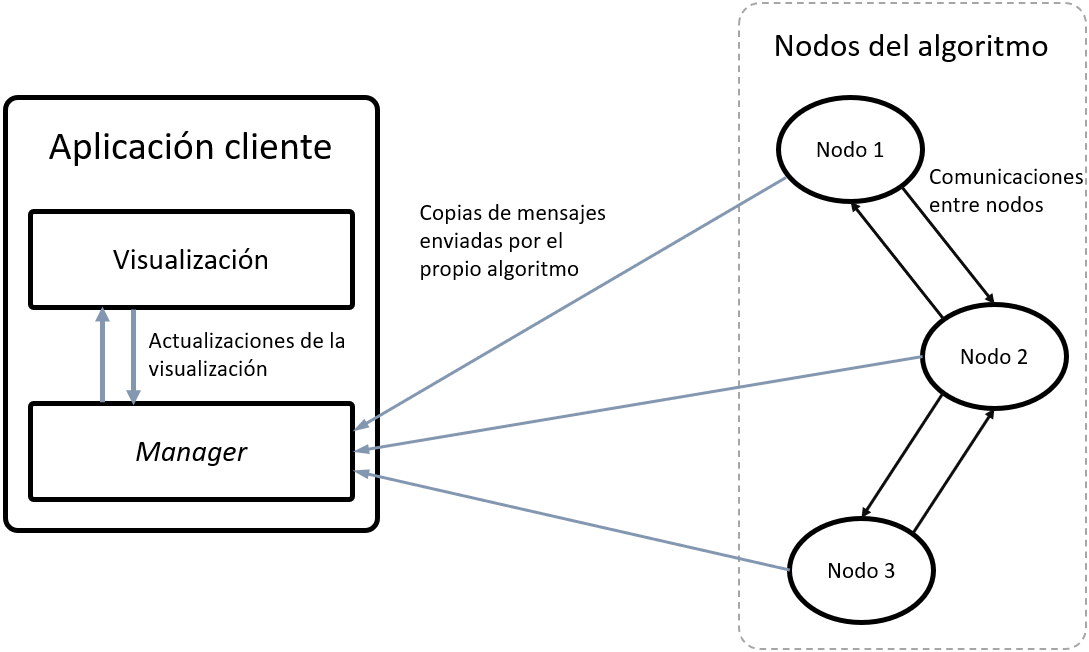
\includegraphics[width=0.7\linewidth]{imagenes/arquitectura1}
  \caption{Diagrama de la primera arquitectura propuesta}
  \label{fig:arquitectura1}
\end{figure}

En la Figura~\ref{fig:arquitectura1} se puede ver en la parte izquierda la aplicación cliente, que se compone de la interfaz, y del proceso \textit{manager} que la actualiza. Ambas partes se ejecutan en la misma máquina. En la parte de la derecha se localizan los nodos del algoritmo, que pueden ejecutarse en un entorno distribuido. Las flechas entre nodos simbolizan las comunicaciones del algoritmo, y las flechas entre cada nodo y el proceso \textit{manager} las copias de los mensajes.

Otra alternativa menos ``intrusiva`` en el algoritmo consiste en modificar de alguna manera las librerías que gestionan los envíos de paquetes de red. De tal forma que el algoritmo llama a la función de librería de envío de mensajes (\texttt{send}, \texttt{sendto}, \texttt{write}, etc) y esta envía una copia del mensaje al proceso \textit{manager}. Esta solución permite no tener que modificar nada del algoritmo. La arquitectura (Figura~\ref{fig:arquitectura2}) es muy parecida a la propuesta anteriormente, lo único que cambia es el origen del envío de las copias de mensajes.

\begin{figure}[h]
  \centering
  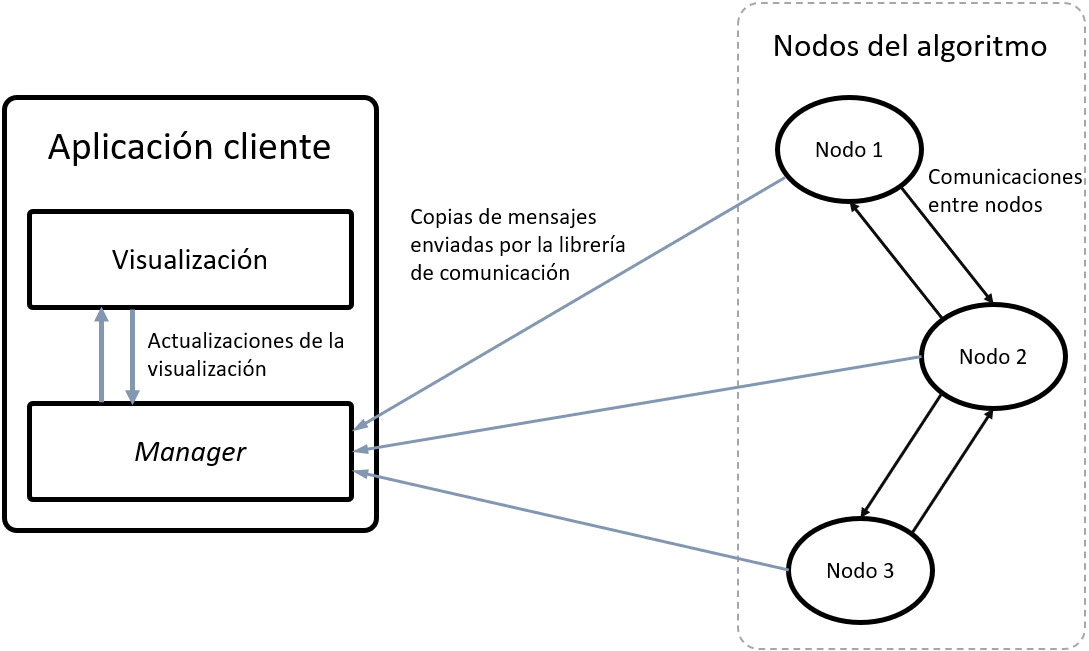
\includegraphics[width=0.7\linewidth]{imagenes/arquitectura2}
  \caption{Diagrama de la segunda arquitectura propuesta}
  \label{fig:arquitectura2}
\end{figure}

\newpage

Sin embargo esta alternativa cuenta con el gran defecto de que no sería posible intercambiar el algoritmo por otro implementado en otro lenguaje de programación cualquiera. Sería necesario volver a modificar las librerías necesarias. Esta resticción, junto con el hecho de que puede ser complicado modificar la funcionalidad incluída en las librerías del lenguaje, motiva la siguiente alternativa.

La alternativa final cuenta con otro proceso capturador o \textit{sniffer} que intercepta el tráfico de red a nivel de protocolo de un determinado proceso. Se ejecuta una instancia junto con cada nodo del algororitmo de tal forma que los mensajes capturados se reenvían al proceso \textit{manager} para que este actualize la visualización. Esta captura de mensajes se lleva a cabo a nivel de protocolo, por lo que no es necesario modificar ningún aspecto del algoritmo que se quiere visualizar. En esta solución el cuadro de mandos se abstrae totalmente del algoritmo, de forma que permite visualizar implementaciones en distrintos lenguajes, siempre que el medio de comunicación sea un protocolo conocido, por ejemplo TCP. Esta modificación se puede observar en la figura~\ref{fig:arquitectura3}.

\begin{figure}[h]
  \centering
  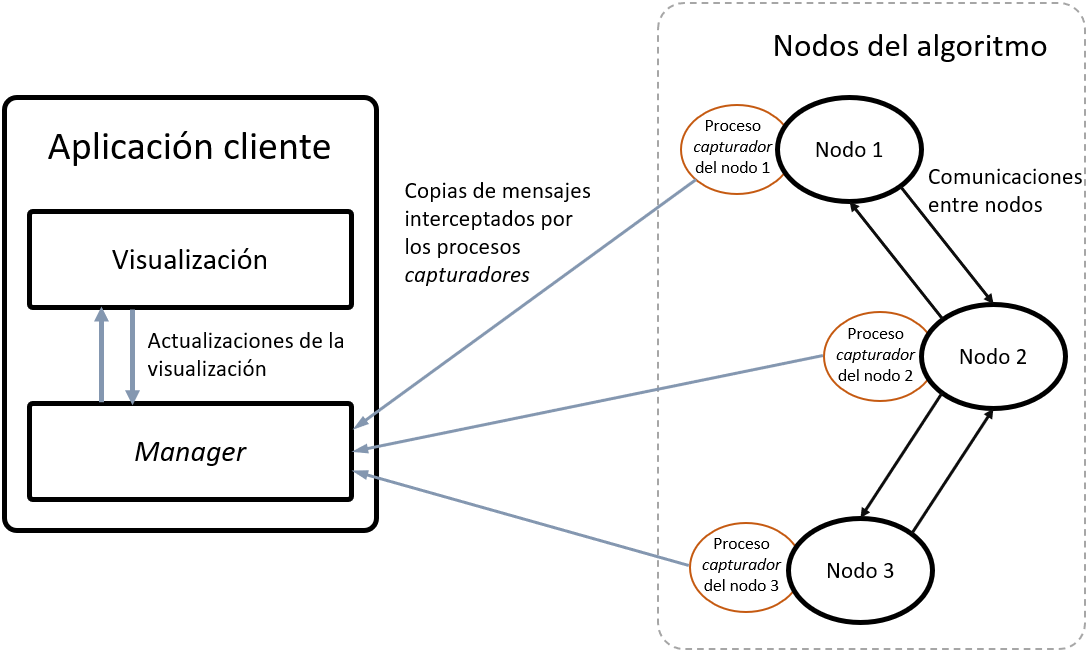
\includegraphics[width=0.7\linewidth]{imagenes/arquitectura3}
  \caption{Diagrama de la tercera arquitectura propuesta}
  \label{fig:arquitectura3}
\end{figure}

Por parte del proceso \textit{manager}, el funcionamiento es el mismo que en las soluciones propuestas anteriormente. Otra ventaja de esta arquitectura es que soportaría también visualizar algoritmos cuyo medio de comunicación se basa en las llamadas a procedimientos remotos (RPC). En las soluciones propuestas anteriores únicamente se tienen en cuenta los algoritmos cuyo modelo de comunicación se basa en el envío de mensajes entre \textit{sockets} (sería necesario modificar el proceso \textit{manger} para admitir la comunicación mediante RPC). Sin embargo, dado que las librerías de llamadas a procedimientos remotos también se basan en la comunicación con algún protocolo (por lo general TCP), también se capturarían estos mensajes.

La ventaja principal de esta arquitectura comparada con las anterior, es que permite un desacoplamiento total del algoritmo. Además de esto, satisface los requisitos que se mencionan en la introducción. A continuación se explicará la implementación detallada de cada uno de los elementos de la arquitectura.

\section{Implementación del proceso \textit{capturador}}

\section{Implementación y descripción del cliente}

\section{Implementación del \textit{manager}}

\section{Caso de uso}

En este apartado se demuestra la funcionalidad completa de la aplicación con un algoritmo concreto: Raft. El funcionamiento de este algoritmo se puede encontrar en el Anexo de este documento. A modo de resumen, Raft es un algoritmo de consenso empleado para replicar información en conjunto de nodos.



\chapter{Análisis de impacto}

En este capítulo se anañizará primero el impacto de los objetivos que se han logrado con este proyecto, clasificándolos según el ámbito al que afectan, y posteriormente se relacionarán con los Objetivos de Desarrollo Sostenible de la ONU.

\section{Impacto personal}

A nivel personal el impacto de este Trabajo de Fin de Grado se ve reflejado sobre todo en la cantidad de conocimientos adquiridos durante la realización del mismo. Estos conocimientos no se basan únicamente en el uso de tecnologías nuevas, si no también en la experiencia que ha supuesto implementar todos los componentes.

\section{Impacto empresarial y económico}

La implementación propuesta es de utilidad para los trabajadores de las empresas que implementan sistemas distribuidos, puesto que facilita el proceso de depuración. Esto implica que los trabajadores pueden completar las tareas de este tipo con mayor velocidad, lo cual tendría una repercusión positiva sobre la empresa.

\section{Impacto cultural}
Además de facilitar la labor de los programadores de aplicaciones distribuidas, este proyecto también mejora la calidad de la docencia en las asignaturas de esta materia. Disponer de un recurso que facilite la explicación de los algoritmos de la materia supone que los estudiantes tendrán más facilidades para comprenderlos.

\section{Relación con los Objetivos de Desarrollo Sostenible}

En 2015 el Ministerio de Derechos Sociales publicó la \textit{Agenda 2030}\cite{agenda2030}, basada en los Objetivos de Desarrollo Sostenible\cite{ods} de la ONU, cuya finalidad es mejorar las condiciones de vida de los ciudadanos. Su nombre se deriva de que en los próximos 15 años (a partir de 2015) el Gobierno debe adoptar medidas para luchar contra el cambio climático y erradicar la pobreza, entre otros. La \textit{Agenda 2030} recoge en 17 apartados los diferentes Objetivos de Desarrollo Sostenible. 

Analizando los objetivos del proyecto, se puede deducir que están estrechamente relacionados con el punto ''Educación de calidad'' de la \textit{Agenda 2030}. Uno de los objetivos principales de este Trabajo de Fin de Grado es proporcionar una herramienta que facilite la docencia en la asignatura de Sistemas Distribuidos y facilite la depuración el ámbito de la programación distribuida. Esto por una parte implicaría una docencia de mayor calidad en las asignaturas de esta materia, y por otra parte tabién mejoraría el desarrollo de aplicaciones distribuidas. Este último aspecto también está relacionado con el punto ''Trabajo Decente y Crecimiento Económico'' de los objetivos de Desarrollo Sostenible, dado que la solución propuesta en este proyecto es una herramienta de apoyo para los programadores de aplicaciones distribuidas, lo cual contribuye a un trabajo de mejor calidad.


\chapter{Conclusiones y trabajo futuro}


%%-----------------------------------------------
%% Bibliografía
\cleardoublepage
\phantomsection
\addcontentsline{toc}{chapter}{Bibliografía}
\bibliographystyle{IEEEtran}
\bibliography{secciones/biblio}

%% -----------------------------------------------
%% Anexos
\appendix
\part*{Anexos}
\addcontentsline{toc}{chapter}{Anexos}
\chapter*{Anexo I - Algoritmo \textit{Raft}}

En materia de Sistemas Distribuidos, uno de los aspectos más dificultosos es mantener la consistencia de los datos en diferentes máquinas. Para lograr esto, se han diseñado numerosos algoritmos, como por ejemplo \textit{Paxos}\cite{paxos} o \textit{Raft}\cite{raft1}. Para este proyecto se ha escogido la implementación de Raft puesto que la implementación, que no deja de ser sencilla, es más sencilla que otros algoritmos, y además la implementación del algoritmo a visualizar no es el objetivo principal. \textit{Raft} es un algoritmo que tiene dos objetivos:

\begin{itemize}
\item Elegir un líder en un conjunto de nodos.
\item Mantener información (\textit{logs}) replicada en múltiples máquinas.
\end{itemize}

Este algoritmo garantiza la integraidad de la información y también ofrece resistencia a comportamiento anóamlo de nodos o caída de estos. Los creadores de este algoritmo, tuvieron como objetivo principal diseñar un algoritmo cuyo funcionamiento sea simple. Previamente a su invención, existían otros algoritmos de este tipo, por ejemplo \textit{Paxos}\cite{paxos}, pero la complejidad de estos impedía que se emplearan extensivamente.

Los nodos que ejecutan el algoritmo \textit{Raft} pueden pertenecer a tres estados: \textit{leader} (líder), \textit{candidate} (candidato) y \textit{follower} (seguidor). Los nodos comienzan su ejecución en el estado \textit{follower}, y dependiendo del estado en el que se encuentre un nodo, ejecuta determinadas operaciones. Por otra parte, cada nodo guarda el \textit{term} en el que se encuentra. Este valor sirve, entre otras cosas, para determinar la antiguedad de los datos de un nodo.

\subsection*{Estado \textit{leader}}

Este estado es el más sencillo, dado que lo único que realiza el nodo es enviar mensajes de tipo \textit{AppendEntries} a los nodos vecinos cada varios decisegundos. A este intervalo de tiempo se le denomina ''\textit{leader heartbeat timeout}''. Estos mensajes contienen las nuevas entradas de \textit{log} que recibe el algoritmo para replicar en todos los nodos. Un nodo deja de ser líder cuando recibe mensajes de otros nodos con un \textit{term} superior. Este escenario significa que el nodo guarda datos antiguos.

\subsection*{Estado \textit{follower}}

Los nodos en el estado \textit{follower} reciben continuamente mensajes de tipo \texttt{AppendEntries} del nodo líder. También cuentan con otro tiempo de \textit{timeout} denominado ''\textit{follower timeout}''. Este tiempo determina el tiempo máximo que puede transcurrir entre dos recepciones de mensajes. Cuando un nodo \textit{follower} deja de recibir mensajes de tipo \textit{AppendEntries} significa que, o bien el líder ha dejado de funcionar, o bien se ha perdido el contacto. Independientemente de la causa del problema, el nodo \textit{follower} pasará al estado \textit{candidate} iniciando una votación. Se podría decir que los nodos en este algoritmo quieren a toda costa convertirse en líderes. Cabe destacar que el tiempo de \textit{timeout} del líder (\textit{leader heartbeat timeout}) debe ser inferior al tiempo de timeout del \textit{follower} (\textit{follower timeout}). Esto es necesario porque si no fuera así, el nodo líder no enviaría a tiempo mensajes \texttt{AppendEntries} a los nodos vecinos, llevándose a cabo una eleción de líder nueva en cada instante.

Además de los mensajes de tipo \texttt{AppendEntries}, tambíen se pueden recibir mensajes de tipo \texttt{RequestVote}. Estos mensajes implican que el nodo acepta la petición de la votación respondiendo con \texttt{GrantVote} si no ha votado ya en el \textit{term} actual.

Por otra parte, si un proceso \textit{follower} recibe mensajes de otro nodo con un \textit{term} superior, se convierte seguidor del nuevo \textit{term}.

\subsection*{Estado \textit{candidate}}

Cuando un nodo \textit{follower} inicia una votación, transita al estado \textit{candidate}, incrementando el \textit{term} actual y enviando mensajes \texttt{RequestVote} a los nodos vecinos. Cuando el nodo recibe $\frac{N + 1}{2}$ mensajes de tipo \texttt{GrantVote}, donde $N$ es el número de nodos vecinos, significa que ha ganado la eleción. En este escenario el nodo transita al estado \textit{leader}.

Si en este estado no se reciben mensajes en un intervalo de tiempo inferior al ''\textit{follower timeout}'', entonces se inicia otra votació nueva incrementando el \textit{term}.

En el caso de que un nodo en el estado \textit{candidate} recibe un mensaje de tipo \texttt{AppendEntries} o \texttt{RequestVote} con un \textit{term} superior, el nodo pasaría inmediatamente al estado \textit{follower}.

\subsection*{Comentarios sobre el algoritmo}

Sobre este algoritmo cabe destacar ciertos aspectos. En primer lugar, dado que cada nodo comienza una votación cada vez que deja de recibir mensajes del líder, es posible que dos nodos en estado \textit{follower} comienzen una votación simultáneamente. Dependiendo del número de nodos del sistema (por ejemplo 4 nodos), se podría dar el caso en el que dos nodos se disputan por ser el líder dado que no reciben suficientes votos, esto iniciaría otra votación y se repetiría el problema indefinidamente. Es por esto por lo que normalmente se establece aleatoriamente el tiempo ''\textit{follower timeout}''. Cuando cada nodo tiene este valor distinto, es muy poco probable que ocurra el escenario mencionado.

Por otra parte se podría dar el caso en el que la red distribuida se divide en dos conjuntos de nodos. En este escenario uno de los conjuntos (que contiene el líder previo) seguiría una ejecuión normal. Sin embargo el otro conjunto elegiría un nuevo líder con un \textit{term} superior. Si se diera el caso en el que los dos conjuntos se conectaran otra vez, el último líder elegido pasaría a ser el líder del grupo, puesto que tiene un \textit{term} superior.














%% ---------------------------------------------------------
\end{document}

%%% Local Variables:
%%% mode: latex
%%% TeX-master: t
%%% End:
